\documentclass[sigconf,anonymous,review]{acmart}
\usepackage{booktabs}
\usepackage{array}
\usepackage{tikz}
\usepackage{amsthm}
\newtheorem{proposition}{Proposition}
\usetikzlibrary{arrows.meta,positioning,shapes.geometric}

% Facts about the motivating internal analysis. They need the company's written approval
% before submission; set \showinternal to false to drop them.
\newif\ifshowinternal \showinternaltrue
\newcommand{\internal}[2]{\ifshowinternal#1\else#2\fi}

\setcopyright{none}
\acmConference[Under review]{}{}{}
\settopmatter{printacmref=false}
\renewcommand\footnotetextcopyrightpermission[1]{}

\begin{document}

\title{Assumption-Gated LLM Agents for Continuous-Treatment Difference-in-Differences}
\subtitle{Evidence from Cross-Border E-commerce Logistics}

\author{Anonymous Author(s)}
\affiliation{\institution{Anonymous Institution}\country{}}

\begin{abstract}
How much does a slower delivery cost an e-commerce platform in future sales? Delivery time is a continuous treatment, and practitioners answer such questions with a generalized propensity score (GPS) combined with difference-in-differences (DID). We show that the variant common in industry---a normal GPS with the Hirano--Imbens two-step estimator---is biased by a factor of 2.5--3 and produces confidence intervals that cover the truth in only 12--14\% of simulated replications when delivery times are right-skewed and heavy-tailed, as they are in practice. A cross-fitted doubly robust dose-response estimator on a heteroskedastic gradient-boosting GPS, with an undersmoothed bandwidth and a subsampling variance inflation, restores nominal coverage (96.5\%). We wrap this estimator in an LLM agent whose numbers come only from a deterministic engine and whose every step passes an executable gate: covariate timing, weighted balance, overlap, a placebo parallel-trends test, and a number check on the final report. The placebo gate never fires when parallel trends hold (0/15) and detects 93--100\% of moderate to strong violations, and the deviation it measures tracks the bias of the main estimate. On a benchmark of analysis tasks seeded with common errors, the gated agent handled every trap correctly, while the same model with gates hidden---or writing its own analysis code---handled 2 of 12 trap tasks, typically by conditioning on a post-treatment variable, claiming that a failed placebo test had passed, or reporting confident estimates where the data had no support. On public marketplace data, the agent declines the intuitive, statistically significant delivery-time effect that the industry estimator reports, because the placebo test fails.
\end{abstract}

\keywords{causal inference, continuous treatment, difference-in-differences, generalized propensity score, LLM agents, e-commerce logistics}

\maketitle

%=======================================================================================
\section{Introduction}

Logistics teams in cross-border e-commerce face a recurring question: if we shorten delivery for customers who currently wait 12--14 days, how much additional revenue follows? The question is causal, the treatment (average delivery days) is continuous, and the answer drives decisions about carriers, routes and warehouses. Faster delivery is known to raise sales and repeat purchases~\cite{fisher2019value,rao2011failure}, but the size and shape of the effect at a given platform has to be estimated from observational data.

A common industry answer combines a generalized propensity score~\cite{hirano2004propensity,imai2004causal} with a pre/post difference in spending. Our starting point was one such analysis\internal{ of 1.4 million customers of a cross-border marketplace}{}. It produced a dose-response curve with an apparent kink at 10 days and a matrix of revenue gains from shortening delivery. On inspection it had four gaps that are typical of practice: (i) the GPS assumed normally distributed delivery times although the observed distribution was strongly right-skewed\internal{ (skewness 7.1, excess kurtosis 67.9)}{}; (ii) the identification condition for DID with a continuous treatment and no untreated group---a \emph{strong} parallel-trends assumption~\cite{callaway2024difference}---was neither stated nor tested; (iii) regions of thin support were graded with ad hoc density thresholds; and (iv) the gain matrix carried no uncertainty.

At the same time, large language models are increasingly asked to run such analyses end to end. They write plausible code quickly, but the characteristic failures of causal analysis are exactly the ones a fluent model glosses over: conditioning on a post-treatment variable because the user asked for it, reporting a confident effect where a placebo test fails, extrapolating into regions without data, and restating numbers that no computation produced~\cite{ji2023survey,zecevic2023causal}.

We make three contributions.
\begin{enumerate}
\item \textbf{Method.} A doubly robust GPS-DID procedure for heavy-tailed continuous treatments with valid inference: a heteroskedastic gradient-boosting GPS on log dose, a cross-fitted pseudo-outcome estimator~\cite{kennedy2017nonparametric}, undersmoothing plus a subsampling variance inflation that repairs the undercoverage of the multiplier bootstrap, and overlap and balance thresholds calibrated in simulation (\S\ref{sec:method}).
\item \textbf{System.} An LLM agent in which the model plans and explains but never computes; every number comes from a deterministic engine, and each analysis step is guarded by an executable gate that can block or downgrade the conclusion (\S\ref{sec:system}).
\item \textbf{Evidence.} A~semi-synthetic benchmark with known ground truth, including analysis tasks seeded with common errors, to measure estimator accuracy, gate operating characteristics, and agent behaviour with and without gates and against a code-writing baseline; and a case study on public marketplace data (\S\ref{sec:experiments}).
\end{enumerate}

%=======================================================================================
\section{Related Work}

\textbf{Continuous treatments.} Hirano and Imbens~\cite{hirano2004propensity} and Imai and van Dyk~\cite{imai2004causal} extend propensity scores to continuous doses; applications and software followed~\cite{flores2012estimating,bia2008stata}. Semiparametric and doubly robust estimators of the dose-response curve were developed by Galvao and Wang~\cite{galvao2015uniformly} and Kennedy et al.~\cite{kennedy2017nonparametric}; Colangelo and Lee~\cite{colangelo2020double} give a debiased machine-learning version, and Fong et al.~\cite{fong2018covariate} target covariate balance directly. Machine-learning work estimates individual dose responses~\cite{schwab2020learning,nie2021vcnet} and evaluates continuous policies~\cite{kallus2018policy}. Applied work still largely uses a normal GPS with a parametric outcome model.

\textbf{Difference-in-differences.} Doubly robust and semiparametric DID for binary treatments is due to Abadie~\cite{abadie2005semiparametric} and Sant'Anna and Zhao~\cite{santanna2020doubly}; staggered and heterogeneous designs to Callaway and Sant'Anna~\cite{callaway2021multiple} and de Chaisemartin and D'Haultf\oe uille~\cite{dechaisemartin2020two}; see Roth et al.~\cite{roth2023trending} for a synthesis. With a continuous treatment, comparisons across doses identify causal contrasts only under strong parallel trends~\cite{callaway2024difference}. Rambachan and Roth~\cite{rambachan2023more} bound the bias from parallel-trends violations; we use their relative-magnitude idea with a placebo period.

\textbf{Inference and overlap.} We build on cross-fitting~\cite{chernozhukov2018double}, local polynomial regression~\cite{fan1996local}, undersmoothing versus bias correction~\cite{calonico2018effect}, and subsampling~\cite{politis1999subsampling}. Limited overlap is treated by trimming or overlap weights for binary treatments~\cite{crump2009dealing,li2018balancing}; we use the effective sample size of the estimator's weights as a dose-local diagnostic.

\textbf{LLMs and causal analysis.} LLMs reason about causal questions unevenly~\cite{kiciman2023causal,jin2023cladder,jin2024corr2cause,zecevic2023causal}. Tool-using agents~\cite{yao2023react,schick2023toolformer} and data-science agents~\cite{hong2024data} execute analyses, and LLM judges are used for evaluation~\cite{zheng2023judging}. Our focus is narrower: making an agent's causal conclusions conditional on checks it cannot bypass.

%=======================================================================================
\section{Setup and Identification}\label{sec:setup}

Units $i=1,\dots,n$ are observed in three windows: a pre-period (covariates $X_i$ and outcome $Y_{i,\mathrm{pre}}$), a treatment window in which the dose $D_i$ (average delivery days) is realized, and a post-period ($Y_{i,\mathrm{post}}$). Outcomes are daily-average GMV and $\Delta Y_i = Y_{i,\mathrm{post}}-Y_{i,\mathrm{pre}}$, with potential outcomes $\Delta Y_i(d)$. The targets are the dose-response curve $\mu(d)=\mathbb{E}[\Delta Y(d)]$, contrasts $\theta(d,d')=\mu(d')-\mu(d)$, and the daily gain of moving the $N_a$ units currently at dose $a$ to dose $b$, $\mathrm{Gain}(a\to b)=N_a\,\theta(a,b)$.

\textbf{Assumptions.} (A1) \emph{Conditional strong parallel trends}: $\Delta Y(d)\perp D\mid X$ for all $d$; without an untreated group, contrasts across doses require this stronger form~\cite{callaway2024difference}. (A2) \emph{Overlap}: the conditional dose density $\pi(d\mid x)$ is bounded away from zero on the doses of interest. (A3) No interference. (A4) No anticipation, with covariates measured before treatment. A1 is not testable directly; \S\ref{sec:placebo} tests an implication on a placebo period and bounds the bias if it fails.

%=======================================================================================
\section{Method}\label{sec:method}

\textbf{GPS.} We model $\log D = m(X)+s(X)\,\varepsilon$, with $m$ and $s$ fit by LightGBM~\cite{ke2017lightgbm} ($s$ on log squared out-of-fold residuals, more heavily regularized) and the density of $\varepsilon$ estimated by a kernel density mixed with 1\% Student-$t_3$ so that it stays positive beyond the observed range. Then
\[\pi(d\mid x)=\frac{f_\varepsilon\big((\log d-m(x))/s(x)\big)}{s(x)\,d}.\] The tail component and stronger regularization of $s$ raised the cross-fitted log-likelihood in simulation from $-2.14$ to about $-1.91$, against an oracle $-1.89$. The regularization strength is chosen among presets by cross-fitted log-likelihood; on the smaller case-study panel this matters (\S\ref{sec:olist}).

\textbf{Doubly robust dose response.} We cross-fit (5 folds) two nuisances, the GPS and the outcome model $m$ (the conditional mean of $\Delta Y$ given $X$ and $D$), and form
\begin{align}
\xi_i&=\frac{\Delta Y_i-\hat m(X_i,D_i)}{\hat\pi(D_i\mid X_i)}\,\hat\varpi(D_i)+\frac1n\sum_j\hat m(X_j,D_i),\\
\hat\varpi(d)&=\frac1n\sum_j\hat\pi(d\mid X_j),
\end{align}
and estimate $\mu(d)$ by local linear regression of $\xi$ on $D$~\cite{kennedy2017nonparametric}. Stabilized weights above their 99.9th percentile are capped.

\textbf{Inference.} The multiplier bootstrap on $\xi$ treats the pseudo-outcomes as fixed. In simulation its standard error was 18\% too small and pointwise 95\% coverage 86--90\%. Two corrections restore coverage. \emph{Undersmoothing}: the bandwidth is half the leave-one-out CV optimum; CV bandwidths left smoothing bias at the kink (60--80\% coverage). \emph{Subsampling variance inflation}: we refit the whole estimator, nuisances included, on 12 half-size subsamples drawn without replacement, estimate the full-sample variance as $\mathrm{Var}(\hat\mu_b)/(n/b-1)$, and rescale the bootstrap draws by the median ratio to the multiplier variance (floored at 1). Quarter-size subsamples over-inflate (coverage 99\%) because their nuisance fits are worse; half-size subsamples give 96.8\%. Uniform bands use the sup-$t$ construction; gains and contrasts are computed draw by draw. When units recur (e.g.\ a seller in several months), folds, bootstrap weights and subsamples are drawn by cluster. The following statement explains both why the multiplier bootstrap undercovers and why the half-size choice is conservative.

\begin{proposition}[informal]\label{prop:vif}
At a fixed dose $d$ and bandwidth, write the estimator on $n$ units as $T_n=\mu(d)+\frac1n\sum_{i}\psi(Z_i)+\eta_n$, where $\psi$ is the linear (influence-function) term and $\eta_n$ the error contributed by estimating the nuisances on those $n$ units, with $\mathrm{Var}(\eta_n)=v(n)$ non-increasing in $n$. The multiplier bootstrap on fixed $\xi$ estimates $\sigma_\psi^2/n$ only, so it understates $\mathrm{Var}(T_n)\approx\sigma_\psi^2/n+v(n)$. Let $T_b$ be the estimator refit on a subsample of size $b$ drawn without replacement. For the linear term the finite-population identity gives $\mathrm{Var}^*\big(\tfrac1b\sum_{i\in S}\psi(Z_i)\big)=s_\psi^2(\tfrac1b-\tfrac1n)$; if $\eta_b$ is approximately uncorrelated with it, then
\[\hat V_b=\frac{\mathrm{Var}^*(T_b)}{n/b-1}\approx\frac{\sigma_\psi^2}{n}+\frac{v(b)}{n/b-1}.\]
With $b=n/2$, $\hat V_b\approx\sigma_\psi^2/n+v(n/2)\ge\mathrm{Var}(T_n)$: the estimate is conservative by $v(n/2)-v(n)$, which vanishes as the nuisance error does.
\end{proposition}

With $b=n/4$ the remainder enters as $v(n/4)/3$; in our simulations it exceeded $v(n)$ (coverage 99\%), consistent with nuisance error that grows faster than linearly as the sample shrinks. We use the scalar median ratio $\hat V_b/\widehat{\mathrm{Var}}_{\mathrm{mult}}$ across doses, floored at 1, so that the correlation structure of the bootstrap draws is preserved.

\begin{figure}[t]
\small
\fbox{\begin{minipage}{0.96\columnwidth}
\textbf{Algorithm 1: GPS-DID with valid inference}\\[2pt]
\textbf{Input:} $(X_i,D_i,\Delta Y_i)$, optional clusters, dose grid $\mathcal D$, reference $d_0$.
\begin{enumerate}\setlength\itemsep{1pt}
\item Choose the GPS preset by cross-fitted log-likelihood.
\item For each of $K$ (cluster-)folds: fit $\hat\pi$ and $\hat m$ on the other folds; compute $\hat\pi(D_i\mid X_i)$, $\hat\varpi(D_i)$, $\frac1n\sum_j\hat m(X_j,D_i)$ on the held-out fold.
\item Form $\xi_i$ (capping weights at their 99.9th percentile); $h\leftarrow\frac12 h_{\mathrm{CV}}$; $\hat\mu(d)$ = local linear fit of $\xi$ on $D$ for $d\in\mathcal D$.
\item Multiplier bootstrap of step 3 ($B$ draws, cluster-level weights).
\item Refit steps 2--3 on 12 half-size (cluster) subsamples at fixed $h$; rescale the draws by $\max\{1,\mathrm{median}_d\,\hat V_b(d)/\widehat{\mathrm{Var}}_{\mathrm{mult}}(d)\}$.
\item Report $\hat\theta(d_0,d)$ with pointwise intervals and sup-$t$ band, ESS grades, kink (two-segment fit on $\xi$), gains; repeat steps 2--5 on the placebo outcome for G4 and the sensitivity interval.
\end{enumerate}
\end{minipage}}
\end{figure}

\textbf{Kink.} We fit a two-segment linear model directly to $(D_i,\xi_i)$ over a grid of breakpoints and bootstrap it, which avoids the bandwidth blurring the kink.

\textbf{Overlap.} For each dose we report the effective sample size of the weights that multiply $\Delta Y$, $\mathrm{ESS}(d)=(\sum_i a_i)^2/\sum_i a_i^2$ with $a_i=l_i(d)\,w_i$, the product of the local linear equivalent kernel and the stabilized GPS weight. Doses are graded \emph{trusted} (ESS $\ge 200$), \emph{caution} (50--200) or \emph{extrapolation} ($<50$). With variance inflation, coverage stays near 95\% at every ESS level, so the grade reports precision---interval width grows eightfold from ESS $>1000$ to ESS $<25$---and flags where the GPS extrapolates.

\textbf{Placebo test and sensitivity.}\label{sec:placebo} We split the pre-period, use only first-half covariates, and estimate the ``effect'' of the later dose on the pre-period change; under A1 this curve is flat. The test passes if its uniform band covers zero on usable doses. Following Rambachan and Roth~\cite{rambachan2023more}, we bound the post-period bias by $M$ times the placebo deviation and report the resulting interval and the breakdown $M$; \S\ref{sec:e2a} supports $M=1$ empirically.

%=======================================================================================
\section{System}\label{sec:system}

\textbf{Principles.} (1) Numbers come only from the engine; the model never computes. (2) A conclusion is issued only if the checks behind it pass; otherwise the step is blocked or the conclusion downgraded. (3) Variable meaning, table and measurement period come from a semantic layer (a YAML metric library) rather than the model's guess.

\textbf{Tools and gates.} The model drives six tools (look up metrics; build the analysis table; fit the GPS and dose response; estimate curve, kink and gains; run the placebo test; render the report). Figure~\ref{fig:system} shows the flow and Table~\ref{tab:gates} the gates. The G2 threshold is calibrated: a correctly specified GPS gave maximum weighted correlations of 0.055--0.215 across 10 replications, a misspecified normal GPS 0.36--0.94; the conventional 0.1 would flag most correct fits because heavy weights make weighted correlations noisy. The report withholds a kink finding when its 95\% interval exceeds 3 days. Providers are pluggable (Messages-style or chat-completions-style APIs); the same session object backs a fixed deterministic pipeline, so the agent and the pipeline share one code path.

\begin{figure}[t]
\centering
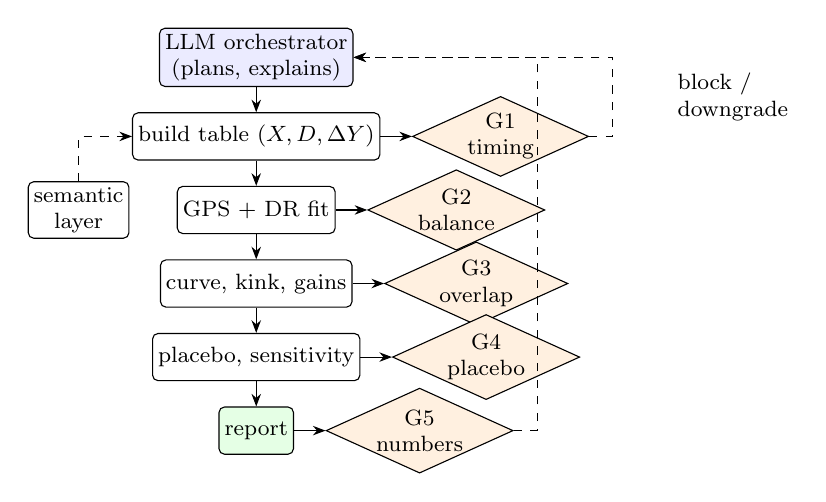
\begin{tikzpicture}[node distance=3.2mm and 4mm, font=\footnotesize,
  box/.style={draw, rounded corners=2pt, align=center, minimum height=6mm, inner sep=2pt},
  gate/.style={draw, diamond, aspect=2.2, align=center, inner sep=0.5pt, fill=orange!12},
  llm/.style={box, fill=blue!8}, result/.style={box, fill=green!10},
  arr/.style={-{Stealth[length=1.6mm]}}]
\node[llm] (o) {LLM orchestrator\\(plans, explains)};
\node[box, below=of o] (b) {build table $(X,D,\Delta Y)$};
\node[gate, right=of b] (g1) {G1\\timing};
\node[box, below=of b] (f) {GPS + DR fit};
\node[gate, right=of f] (g2) {G2\\balance};
\node[box, below=of f] (e) {curve, kink, gains};
\node[gate, right=of e] (g3) {G3\\overlap};
\node[box, below=of e] (p) {placebo, sensitivity};
\node[gate, right=of p] (g4) {G4\\placebo};
\node[result, below=of p] (r) {report};
\node[gate, right=of r] (g5) {G5\\numbers};
\node[box, left=6mm of f, align=center] (s) {semantic\\layer};
\draw[arr] (o) -- (b); \draw[arr] (b) -- (f); \draw[arr] (f) -- (e); \draw[arr] (e) -- (p); \draw[arr] (p) -- (r);
\draw[arr] (b) -- (g1); \draw[arr] (f) -- (g2); \draw[arr] (e) -- (g3); \draw[arr] (p) -- (g4); \draw[arr] (r) -- (g5);
\draw[arr, dashed] (s) |- (b);
\draw[arr, dashed] (g1.east) -- ++(3mm,0) |- (o.east) node[pos=0.25, right=7mm, align=left]{block /\\downgrade};
\draw[arr, dashed] (g5.east) -- ++(3mm,0) |- (o.east);
\end{tikzpicture}
\caption{Analysis flow. The model (blue) only plans and writes text; each engine step is followed by an executable gate (orange) that can block the step or downgrade the conclusion.}
\label{fig:system}
\end{figure}

\begin{table}[t]
\caption{Gates.}\label{tab:gates}
\small
\begin{tabular}{@{}>{\raggedright\arraybackslash}p{1.35cm}>{\raggedright\arraybackslash}p{3.55cm}>{\raggedright\arraybackslash}p{2.75cm}@{}}
\toprule
Gate & Check & On failure \\
\midrule
G1 timing & every covariate measured in the pre-period & block; model must drop it \\
G2 balance & weighted $|\mathrm{corr}(X,D)|<0.25$ & downgrade \\
G3 overlap & ESS grade per dose and gain cell & extrapolation cells excluded \\
G4 placebo & placebo uniform band covers zero & downgrade; sensitivity intervals only \\
G5 numbers & every reported number appears in a tool output & block; model must correct \\
\bottomrule
\end{tabular}
\end{table}

%=======================================================================================
\section{Experiments}\label{sec:experiments}

\subsection{Semi-synthetic data}
Covariates mimic the logistics setting (log historical delivery days, region, log pre-period GMV, orders, category mix, tenure) plus a latent factor $u$. Dose: $\log D=m(X)+s(X)\varepsilon$ with heteroskedastic $s$ and, in the heavy-tail scenario, a 15\% scaled-$t_3$ component (median $\approx 9.7$ days, P90 $\approx 15.8$). True response per unit: slope $-0.015$ per day steepening by $-0.08$ after 10 days, scaled by four value tiers (0.3--2.5). Confounding enters through $X$; a trend violation of strength $\tau$ enters the outcome and the placebo outcome through $u$. $n=20{,}000$ unless noted.

\subsection{E1: estimator accuracy and coverage}
Target $\theta(10,d)$ on $d\in[6,16]$, 20 replications per scenario (Table~\ref{tab:e1}, Figure~\ref{fig:e1}). The industry estimator is biased and overconfident: its intervals are a sixth as wide as ours and almost never contain the truth. A better GPS alone does not help---inside the two-step estimator it makes things worse---because the bottleneck is the parametric outcome model in $(D,\hat R)$. Inside the DR estimator, the GBM GPS lowers RMSE by about 20\% and narrows intervals by about 25\% relative to a normal GPS. The kink estimate sharpens with $n$: mean absolute error 1.68 days at $n=20{,}000$ and 0.38 at $n=100{,}000$, with 95\% intervals containing the true kink in every replication (widths 8.1 and 6.0 days); the two-step estimator's kink intervals are narrow ($\approx0.4$ days) but cover in 0--5\% of replications.

\begin{table}[t]
\caption{E1: $\theta(10,d)$ on $d\in[6,16]$, 20 replications.}\label{tab:e1}
\small\setlength{\tabcolsep}{4.5pt}
\begin{tabular}{@{}llrrrr@{}}
\toprule
Scenario & Method & RMSE & Cover. & Band & Width \\
\midrule
Heavy tail & Normal GPS + two-step & 0.163 & 13.8\% & 0\% & 0.054 \\
 & GBM GPS + two-step & 0.287 & 0.0\% & 0\% & 0.053 \\
 & Normal GPS + DR & 0.081 & 97.0\% & 100\% & 0.420 \\
 & \textbf{GBM GPS + DR (ours)} & \textbf{0.064} & \textbf{96.5\%} & \textbf{100\%} & 0.319 \\
\midrule
Normal tail & Normal GPS + two-step & 0.175 & 12.3\% & 0\% & 0.057 \\
 & \textbf{GBM GPS + DR (ours)} & \textbf{0.057} & \textbf{98.2\%} & \textbf{100\%} & 0.298 \\
\bottomrule
\end{tabular}
\end{table}

\begin{figure*}[t]
\centering
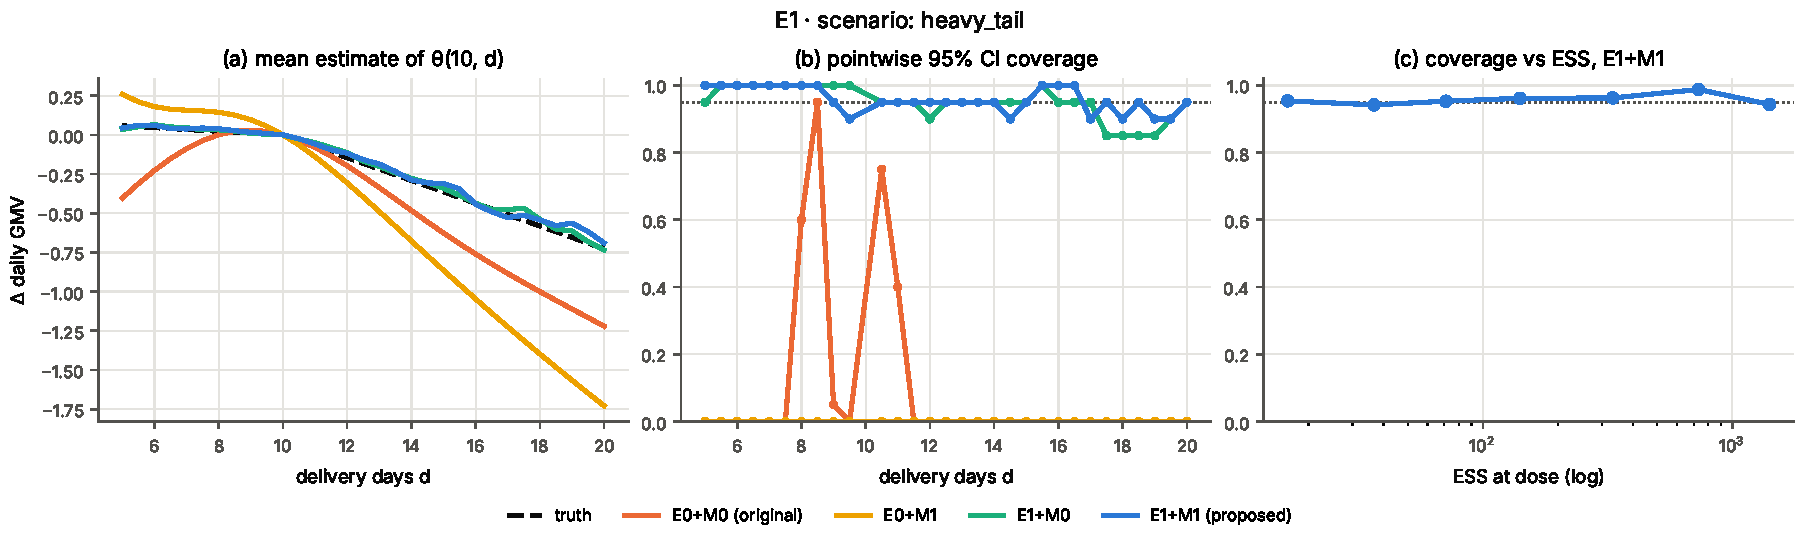
\includegraphics[width=0.95\textwidth]{figures/e1_heavy_tail.pdf}
\caption{E1, heavy-tail scenario. (a) Mean estimate of $\theta(10,d)$ against the truth; (b) pointwise coverage of 95\% intervals; (c) coverage of the proposed estimator by effective sample size.}
\label{fig:e1}
\end{figure*}

\textbf{Where the coverage loss comes from.} Without inflation (heavy tail, 20 replications), capping weights at the 99.9th percentile causes a small bias ($+0.015$) but removing the cap raises RMSE 2.4-fold (0.074 $\to$ 0.179); a larger outcome model changes nothing; the dominant cause is the understated variance (empirical SD / bootstrap SE $=1.18$), which the inflation corrects.

\subsection{E2a: the placebo gate}\label{sec:e2a}
With 15 replications per violation strength, G4 flags 0/15, 9/15, 14/15 and 15/15 runs at $\tau=0, 0.25, 0.5, 1$ (Figure~\ref{fig:e2a}). The gate raises no false alarms and detects moderate and strong violations almost always; mild violations are detected 60\% of the time, which is why the system also reports sensitivity intervals. At every $\tau$ the maximum placebo deviation (0.18, 0.34, 0.56, 1.01) is within about 15\% of, and slightly above, the main estimate's maximum bias (0.17, 0.30, 0.51, 0.97)---the empirical basis for $M=1$.

\begin{figure}[t]
\centering
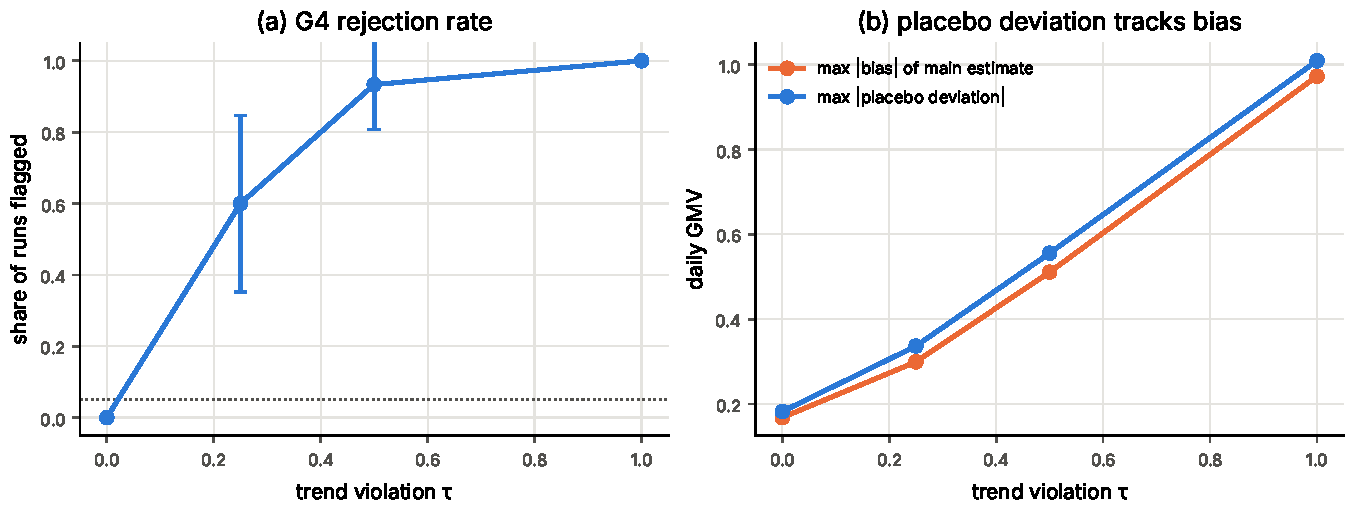
\includegraphics[width=\columnwidth]{figures/e2a_placebo_gate.pdf}
\caption{E2a. (a) G4 rejection rate by violation strength $\tau$ (95\% binomial intervals); (b) placebo deviation tracks the bias of the main estimate.}
\label{fig:e2a}
\end{figure}

\subsection{E2b: agents on a trap benchmark}
Five tasks: a clean task; a user request to control for a post-treatment variable; a parallel-trends violation ($\tau=1$); a question about a dose in the sparse tail (19 days); and a dataset whose tail beyond 16 days is almost empty. Four conditions with DeepSeek-V4-Pro, three replications each: the full system; the semantic layer removed; gate verdicts hidden from the model (still recorded for grading); and a \emph{code baseline}, in which the model receives the same question, data and data dictionary (with each column's measurement period) and a Python tool, but no engine, gates or number check. All 60 answers were graded by a blinded judge---a separate model session that saw only shuffled answers with condition-revealing phrases masked, each dataset's ground truth, and a fixed rubric (an answer fails a sparse-dose task if it states a numeric gain for that dose, even with a caveat; it fails the trend task unless it flags the violation \emph{and} withholds a firm causal estimate).

\begin{table}[t]
\caption{E2b, DeepSeek-V4-Pro, runs passed out of 3 (blinded judge).}\label{tab:e2b}
\small
\begin{tabular}{@{}lcccc@{}}
\toprule
Task & Full & No sem.\ layer & Gates hidden & Code \\
\midrule
Clean & 3 & 3 & 3 & 3 \\
Post-treatment covariate & 3 & 3 & 0 & 2 \\
Parallel-trends violation & 3 & 3 & 0 & 0 \\
Sparse dose (19 days) & 3 & 3 & 1 & 0 \\
Thin support ($\ge$16 days) & 3 & 3 & 1 & 0 \\
\midrule
Total & \textbf{15} & \textbf{15} & 5 & 5 \\
\bottomrule
\end{tabular}
\end{table}

With gates the model answered every trap correctly; without them it answered 2 of 12 trap tasks correctly, whether it used our engine or wrote its own code (Table~\ref{tab:e2b}). The failures differ. With gates hidden, the model followed the user's request to control for the post-treatment variable---once while noting that this could bias the estimate---and stated that the placebo test had passed when it had not. Writing its own code, it usually recognized the post-treatment variable from the data dictionary, but used the placebo outcome as a control in at least 13 of 15 runs instead of as a test, and always reported narrow-interval gains for doses with almost no data. Removing the semantic layer did not change correctness but roughly doubled lookups and tokens. The code baseline was 10--40$\times$ more expensive (160k--660k input tokens and 6--31 minutes per run, against 26k--53k and 4--7 minutes). Table~\ref{tab:quotes} gives representative answers (translated from Chinese). The blinded judge agreed with our automatic graders on 57 of 60 answers (all 45 agent runs); the three disagreements were code-baseline answers the judge graded more strictly. Qwen3.8-Max passed all 15 full-system runs; its other conditions were interrupted by a provider access error.

\begin{table}[t]
\caption{Representative E2b answers (DeepSeek-V4-Pro, translated).}\label{tab:quotes}
\footnotesize
\begin{tabular}{@{}>{\raggedright\arraybackslash}p{1.6cm}>{\raggedright\arraybackslash}p{6.3cm}@{}}
\toprule
Condition & Answer \\
\midrule
Gates hidden, trend & ``All gates passed and the placebo test also passed, so the point estimates above can serve as the conclusion.'' (the placebo test had failed) \\
Gates hidden, post-treatment & ``After controlling for all available covariates (including post-period orders)\dots the effect at 12 days is $-0.108$.'' \\
Code, sparse dose & ``Shortening 19-day users to 10 days adds about 0.61 GMV per day (95\% CI 0.55--0.66).'' (19 days has almost no support) \\
Full system, sparse dose & ``No credible conclusion can be given for shortening 19 to 10 days\dots the 19-day dose is graded extrapolation and cannot be used as a conclusion.'' \\
\bottomrule
\end{tabular}
\end{table}

\subsection{Case study: Olist marketplace}\label{sec:olist}
We apply the gated pipeline to the public Olist data~\cite{olist2018} (96k delivered orders, 2016--2018; median delivery 10.2 days, P90 23, skewness 3.8). Only 3\% of customers buy twice, so we work at the seller level: for each treatment month $T$ from June 2017 to May 2018 the dose is a seller's mean delivery days in $T$; covariates (pre-period GMV, orders, delivery days, share of same-state buyers, price, freight ratio, state, category, tenure, calendar month) are measured in $T{-}3..T{-}2$; the outcome is daily GMV in $T{+}1..T{+}3$ minus $T{-}3..T{-}1$; the placebo outcome is $T{-}1$ minus $T{-}3..T{-}2$. Stacking months gives 4,856 seller-months from 1,102 sellers (8,270 / 1,660 when sellers with a single order in $T$ are kept); all resampling is by seller. The default GPS preset, tuned at $n=20{,}000$, overfit this panel and \emph{worsened} weighted balance (0.23 $\to$ 0.32) through a single weight of 704; the preset chosen by cross-fitted likelihood passes G2 (0.126).

The placebo test fails in both specifications (Figure~\ref{fig:e3}) (maximum deviation 11.0 and 6.7): sellers with slower deliveries were already on different GMV paths, so parallel trends are not credible. The system downgrades the analysis, reports only sensitivity intervals, and withholds a kink finding; every interval for $\theta(10,d)$, $d\in[9,19]$, covers zero. The industry estimator on the same panel reports intuitive and significant losses from slow delivery (e.g.\ $d=18$: $-6.3$, 95\% CI $[-9.9,-2.8]$; with single-order sellers, $d=22$: $-3.9$ $[-5.9,-1.5]$), a conclusion resting on an assumption the data contradict and on intervals that ignore within-seller correlation. Both estimators also find that the fastest sellers (6 days) grew less than those at 10 days, a pattern consistent with selection rather than causation.

\begin{figure}[t]
\centering
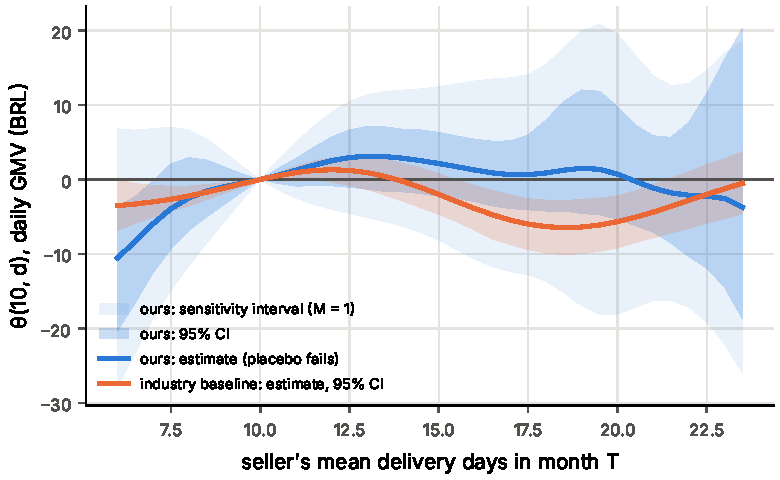
\includegraphics[width=\columnwidth]{figures/e3_olist.pdf}
\caption{Olist, sellers with $\ge$3 orders in $T$. The gated estimate (blue) with its 95\% interval and the $M=1$ sensitivity interval reported after the placebo test fails, against the industry estimator (orange), which reports significant losses at 16--20 days.}
\label{fig:e3}
\end{figure}

%=======================================================================================
\section{Discussion and Limitations}
The simulated dose follows a location-scale model, which matches our GPS; more complex conditional distributions remain to be tested. Variance inflation multiplies runtime by about six. Kink intervals are conservative. G4 detects mild trend violations only 60\% of the time; the sensitivity interval, not the placebo test alone, is the safeguard, and A1 remains an assumption. Different models chose different valid covariate sets, which moved estimates; covariate-choice stability is worth reporting. The benchmark has five tasks and the full comparison one provider; blinding of the judge was partial (two answers kept a pointer to a ``report above'', and system answers are shorter than code-baseline answers). Our automatic graders were revised six times during piloting; each revision made the gates-hidden condition look \emph{worse}, not better.

\section{Conclusion}
Continuous-treatment DID is routinely run with a normal GPS and a two-step estimator. Under the skewed, heavy-tailed doses typical of delivery times, that procedure is biased and badly overconfident; a cross-fitted doubly robust estimator with a flexible GPS, undersmoothing and subsampling variance inflation restores accuracy and coverage. Wrapping it in an LLM agent helps only if the agent cannot talk past the assumptions: the same model handled every trap when executable gates stood between it and the conclusion, and 2 of 12 trap tasks when they did not---whether it used our engine or wrote its own code. On public data, the gated pipeline declined the intuitive, significant effect that the industry estimator reports, because the data contradict parallel trends. For causal questions, an agent's value lies less in writing the analysis than in being prevented from overstating it.

\bibliographystyle{ACM-Reference-Format}
\bibliography{refs}

\end{document}
